\chapter{Polarimetric Calibration}
\label{chapter:polcal}

Hypothetically, integrating over long observing seasons should average-down the noise in the EoR window, allowing for the study of the EoR without the risk of foreground contamination. However, the wedge-window paradigm arises due to the chromaticity of the interferometer as well as the signal. Spectral structure can be imparted to interferometric visibilities by the frequency evolution of the antenna beam and by calibration. Spectral structure can also be induced on otherwise-smooth foregrounds via Faraday rotation of polarized foregrounds. In of itself Faraday rotation is not a problem, since {\sc hi} emission should be largely unpolarized, but errors in calibration and beam deconvolution can leak polarized signal into unpolarized visibilities \citep[e.g.][; Chapter~\ref{chapter:interferometry}]{TMS}.

Interferometers with $N$ antennae that are sensitive to $N_{\rm pol}$ polarizations will generate $N_{\rm pol}N(N-1)/2$ visibilities per time-frequency sample, defined as:

\begin{eqnarray}
V_{ij,pq}(\nu, t) = g^*_{p,i}(\nu,t) g_{q,j}(\nu,t) \exp(-2\pi\nu \tau_{pq}) \times \nonumber\\
\int {\rm d}\Omega A_{pq}(\nu, \hat{s}) S_{P}(\nu, \hat{s}) \exp(i \vec{b}_{ij}\cdot\hat{s} \nu/c)
\end{eqnarray}

where $p,q \in x,y$ denote instrumental polarizations, i.e. the response to signal projected into the North-South direction or the East-West direction, or whichever direction the dipole arms of the instrument are oriented; $i,j$ refers to two antennae with baseline vector $\vec{b}_{ij}$, $S_{P}(\nu, \hat{s})$ is the sky temperature for Stokes parameter $P$, and $A_{pq}(nu, \hat{s})$ is the spatial sensitivity of the instrument to $S_{P}$ (projected into the instrumental basis). Outside the integral are three direction-independent variables that must be calibrated: the complex gain of each dipole arm $g_{p,i}(\nu,t)$ and the phase between dipole arm $p$ and $q$, $\tau_{pq}$. For $p=q$, $\tau_{pq}=0$.

All the above presents a data processing challenge: these visibilities must be precisely calibrated over long observing seasons to ensure that the cosmological signal is not averaged away by calibration errors and not contaminated by spectral structure. One way of overcoming part of this challenge is to construct large arrays of redundantly-spaced elements. The redundancy of the visibilities of such an interferometer allows the gain terms to be solved-for precisely by least-squares minimization algorithms \citep{Liu.10}. In Section~\ref{sec:polcal_redcal}, I explore the implications of implementing full-polarization redundant calibration on PAPER-128 data. However, redundant calibration is not the only tool radio astronomers posses that can be used to obtain precise calibration solutions. In Section~\ref{sec:polcal_imagecal}, I present a basic implementation of full-polarization image-based calibration on data from the PAPER-32 polarized imaging array.

\section{Redundant Calibration}
\label{sec:polcal_redcal}

Unpolarized redundant calibration has been pursued by the Donald C. Backer Precision Array for Probing the Epoch of Reionization (PAPER; \citet{Parsons.10}), the Hydrogen Epoch of Reionization Array (HERA; \citet{deBoer.17}) and part of the Murchison Widefield Array (MWA; \citet{Tingay.13}). For EoR studies this has the advantage of being able to average-down noise in the EoR window once all redundant visibilities are calibrated, for potentially very high signal-to-noise measurements of narrow regions of \textit{k}-space. However, it sacrifices $uv$-coverage, leading to poor imaging capabilities.

Redundant calibration of low-frequency interferometers has been demonstrated by \citet{Zheng.14} with the MIT EoR experiment, \citet{Parsons.14, Jacobs.15, Ali.15}  and {\color{red} Kolopanis et al. (2018)} with PAPER and {\color{red} Li et al. 2017} with part of the MWA. All of these studies calibrated linearly-polarized instrumental visibilities. 

\citet{Moore.17} used the same calibration parameters as \citet{Parsons.14} and \citet{Jacobs.15}, but also solved for a single value of $\tau_{pq}$ for the observing season, since their analysis was for cross-polarized visibilities also. These PAPER studies took linear combinations of instrumental visibilities to form `pseudo-Stokes' visibilities (e.g. \citet{TMS}, \citet{Moore.13}). In this Chapter, we use the notation and convention

\begin{equation}
\left(\begin{array}{c}
V_{I}\\
V_{Q}\\
V_{U}\\
V_{V}\end{array} \right)
= \frac{1}{2}
\left( \begin{array}{cccc}
1 & 0 & 0 & 1 \\
1 & 0 & 0 & -1 \\
0 & 1 & 1 & 0 \\
0 & -i & i & 0 \end{array} \right) 
\left(\begin{array}{c}
V_{xx}\\
V_{xy}\\
V_{yx}\\
V_{yy}\end{array} \right) 
\label{eq:polcal_pseudo-stokes}
\end{equation}
for these quantities.

As noted above, the spectrally-structured HI emission from the EoR should only be detected in $V_{I}$, but fractions of Faraday-rotated (spectrally structured) $V_{Q}$ and $V_{U}$ are capable of leaking into $V_{I}$ via calibration errors and intrinsic properties of the complex beam. Short of detecting the polarized power spectrum of $V_{Q}$ and $V_{U}$, which may be at levels beneath the EoR signal, we require confidence that we are accurately calibrating our data to prevent as much leakage as possible into $V_{I}$. 

At these low frequencies and inherently large scales probed by modern instruments, the Stokes V sky appears to be empty. Indeed, \citet{Patil.17} used the spherical power spectra of their Stokes V images as a proxy for the thermal noise power spectrum. In wedge-space, one test of polarimetric calibration is therefore to see how close to thermal noise $V_{V}$ is. 
\citet{Kohn.16} observed a direction-independent bias in $V_{V}$, but that study implemented a \citet{Moore.17}-style polarimetric calibration of $\tau_{pq}$, solving for a single value across the array, which could indeed lead to a direction-independent bias (but was more powerful than not calibrating it at all; see their Figure 5).

In Section, we explore different schemes of redundant calibration which include polarization. We present three different calibration schemes, all based around the {\sc omnical}\footnote{\url{https://github.com/HERA-Team/omnical}} package \citep{Zheng.14}, and compare their uses and shortcomings. We structure the discussion as follows: in Section~\ref{sec:polcal_math} we give a mathematical overview of the least-squares minimization algorithms implemented for the different calibration schemes and show basic simulations of each algorithm in action. We describe the real data used to test the calibration schemes, and the results of those tests, in Sections~\ref{sec:polcal_data} and \ref{sec:polcal_results}, respectively. We discuss our findings and conclude in Section~\ref{sec:polcal_disc}.

\subsection{Mathematical Overview}
\label{sec:polcal_math}

In this section we briefly describe the fundamental steps of the redundant calibration scheme implemented in {\sc omnical}. For a more thorough discussion of the algorithm, see \citet{Wieringa.92}, \citet{Liu.10}, \citet{Zheng.14} and \citet{Dillon.17}. 

\subsubsection{Redundant calibration with {\sc omnical}}

We can express visibilities for baseline separation $|i-j|$, polarization $pq$ as a system of equations, of form

\begin{equation}
V_{ij,pq} = g^*_{p,i} g_{q,j} V_{|i-j|,pq} + n_{ij}
\label{eqn:vismdl}
\end{equation}

where we have dropped the frequency and time dependence; this is true for every time-frequency sample. This system is overdetermined for a highly redundant array configuration. We assume that all polarizations have the same noise statistics for noise $n_{ij}$. An initial estimate for the least-squares fit can be obtained by solving the linearized equation in logarithmic space (termed \textit{logcal})

\begin{equation}
\log V_{ij,pq} = \log g^*_{p,i} + \log g_{q,j} + \log V_{|i-j|,pq}
\label{eqn:logcal}
\end{equation}

which can constrain the parameter space, but produces biased results since noise is additive in linear space. Taylor expanding Equation~\ref{eqn:vismdl} around the estimated values (denoted with bars) for each parameter as found by \ref{eqn:logcal} grants a system of linearized equations (termed \textit{lincal})

\begin{eqnarray}
V_{ij,pq} = \bar{g}^*_{p,i} \bar{g}_{q,j} \bar{V}_{|i-j|} + g^*_{p,i} \bar{g}_{q,j} \bar{V}_{|i-j|} + \nonumber\\
 \bar{g}^*_{p,i} g_{q,j} \bar{V}_{|i-j|} + \bar{g}*_{p,i} \bar{g}_{q,j} V_{|i-j|}
\end{eqnarray} 

which can be solved iteratively, minimizing the least-squares statistic $w$

\begin{equation}
w^2 = \sum_{\rm{all } i \neq j} \sum_{p,q \in x,y}\frac{|V_{ij,pq} -  g^*_{p,i} g_{q,j} V_{|i-j|,pq}|^2}{\sigma_{ij}}.
\label{eq:polcal_w2}
\end{equation}

\subsubsection{Including polarization in redundant calibration}
\label{subsec:calSchemes}

We test three different calibration schemes for polarization. 

\begin{itemize}
\item Use {\sc omnical} separately on the two linearly polarized visibilities $V_{xx}$ and $V_{yy}$ to obtain independent estimates for all gain terms, and apply those gains to all four instrumental polarizations of visibilities. We will refer to this scheme as \textit{2pol} calibration. 

\item Include all four instrumental polarizations in the least-squares statistic. This means that, for example, information on the $g_{x,i}$ term will come from $V_{xx}$ and $V_{xy}$. This will be referred to as \textit{4pol} calibration. 

\item Use a scheme in which the cross-polarized visibilities $V_{xy}$ and $V_{yx}$ share values of the model visibility $V_{|i-j|,pq}$. This means that we are minimizing the value of $V_{yx} - V_{xy}$ during calibration; effectively minimizing the pseudo-Stokes V visibility. There is validity to assuming the pseudo-Stokes V visibility to be noise-like, as discussed above. We refer to this calibration scheme as \textit{4pol+minV} calibration.
\end{itemize} 

\subsubsection{Degeneracies}
\label{subsubsec:degen}

One virtue of {\sc omnical} is that it can calibrate all antennas relative to one another without reference to an explicit sky model. However, this results in known degeneracies in the minimization of $w^2$ that cannot be resolved with {\sc omnical} and must be fixed afterwards with absolute calibration of the whole array using external information. The number of degeneracies is equal to the number of zero eigenvalues that arise in the linearized $w^2$ minimization algorithm. For a single polarization, there are 4 degenerate modes, which can be interpreted physically as overall amplitude, overall phase, phase tilt, and phase tip. Phase tilt and tip can be interpreted as a two-dimensional phase slope across the array. It is clear that these factors to not affect the product $g^*_{p,i}(\nu,t) g_{q,j}(\nu,t)V_{ij,pq}(\nu, t)$ (and we again refer the reader to \cite{Dillon.17} for a comprehensive description):

\begin{itemize}
\item Overall amplitude: $g_{p,i} \rightarrow A g_{p,i}$ and $V_{ij,pq} \rightarrow V_{ij,pq}/A^2$.
\item Overall phase: $g_{p,i} \rightarrow g_{p,i}e^{i\phi}$
\item Two-dimensional phase slope: for a co-planar array, define a phase vector $\vec{\Upsilon} = (\Upsilon_X,\Upsilon_Y)$ where $\Upsilon_X,\Upsilon_Y$ refer to Cartesian directions as opposed to polarizations. For an antenna at position $\vec{\upsilon}_i$, and defining $\vec{d}_{ij} = \vec{\upsilon}_i - \vec{\upsilon}_j$, then $g_{p,i} \rightarrow g_{p,i}e^{i\vec{\Upsilon}\cdot\vec{\upsilon}_i}$ and $V_{ij,pq} \rightarrow V_{ij,pq}e^{i\vec{\Upsilon}\cdot\vec{d}_{ij}}$. This is allowed because $\vec{d}_{ij}$ is the same for all redundant visibilities.
\end{itemize}

{\sc omnical} `fixes' the amount that the amplitude degeneracy is able to drift between samples by imposing that the average of the absolute of the gains over the array average to unity. Similar tricks can be played with the other degeneracies to project them into a space that does not adversely effect calibration.

The phenomenon of `degeneracy fixing' in polarized redundant calibration was explored in depth by \citet{Dillon.17}. In that work, they showed how the number of degeneracies changes with polarized calibration scheme, focussing on what we refer to as the \textit{2pol} and \textit{4pol} schemes in this work. We briefly review their results here. 

In the \textit{2pol} scheme, there are the 8 expected redundancies as expected for two independent calibrations; it is as if there are two co-located arrays for $xx$ and $yy$, each with the four degeneracies listed above. However, in the \textit{4pol} scheme, the number of degeneracies is reduced to 6. Introducing $V_{xy}$ and $V_{yx}$ breaks the phase tilt and tip degeneracies per polarization, and leaving a polarization-independent phase tilt and tip. Extending this formalism to the \textit{4pol+minV} scheme\footnote{As explored in the public HERA Memo \#30.}, the number of degeneracies is further reduced to 5. By imposing equality between $V_{xy}$ and $V_{yx}$, the `overall phase' degeneracies per polarization are broken and there remains only a single overall phase for the array.

\citet{Dillon.17} emphasized the importance of understanding how fixing degeneracies can effect the amplitude of noise in redundant calibration solutions. They found that although the number of degeneracies decreased in the \textit{4pol} scheme, $V_{xy}$ and $V_{yx}$ had low enough signal to noise that their inclusion in calibration greatly increased the noise in the gain solutions. Fixing only the 6 degeneracies of that scheme introduced much greater noise amplitude in the calibration solutions. However, fixing the 8 degeneracies from the \textit{2pol} scheme \textit{while still calibrating} with the \textit{4pol} scheme gave almost identical gain solutions. Learning from this, we fix the 8 degeneracies from the \textit{2pol} scheme throughout the rest of this work, independent of the calibration scheme used.

\subsubsection{Expectations from simulation}  

Using the formalism of \cite{Nunhokee.17} and Chapter~\ref{chapter:interferometry}, and the HFSS\footnote{\url{http://www.ansys.com/Products/Electronics/ANSYS-HFSS}} complex voltage simulations of the PAPER beam described therein, we simulated the polarized response of the instrument to an unpolarized sky. That is, we passed a Stokes I - only sky model \citep[][]{GSM.08} over a 30\,m East-West baseline -- the baseline vector of interest for the PAPER experiment \citep{Parsons.14, Jacobs.15, Ali.15, Moore.17}. This means that whatever was observed in the pseudo-Stokes Q, U and V visibilities could be interpreted as direction-dependent leakage from Stokes I (the expected regime for a single night of observations with PAPER; \citealt{Kohn.16}). The 2008 Global Sky Model used for the simulation was primarily diffuse in nature, with the `A-Team' of bright low-frequency sources (Fornax A, Pictor A, etc.) also included. The diffuse nature was appropriate for the fringe profile of a 30\,m baseline. The output of the simulation is shown in Figure~\ref{fig:simvis} with and without the inclusion of an instrumental noise model, with the system noise drawn from \cite{Moore.17}.

\begin{figure}
\centering
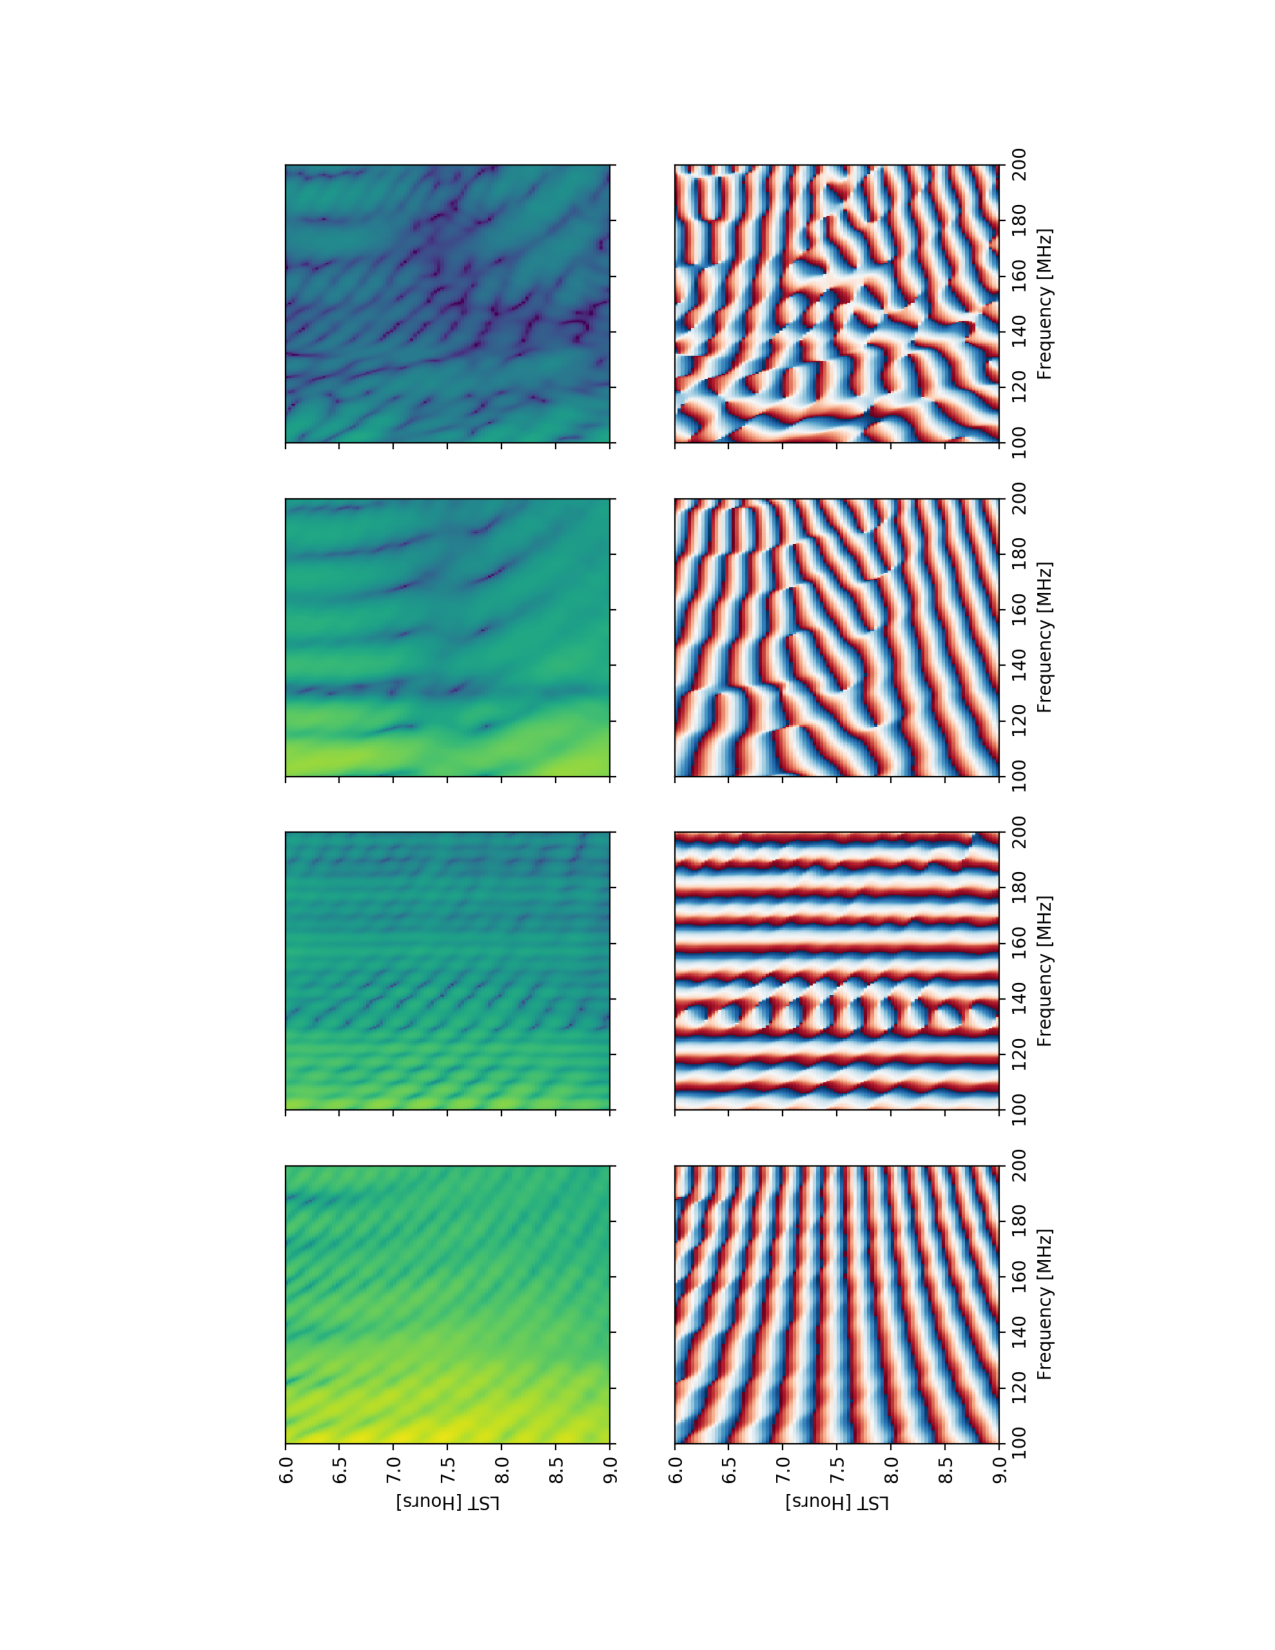
\includegraphics[width=0.6\textwidth, angle=270]{chapters/polcal/figures/sim_nonoise.pdf}
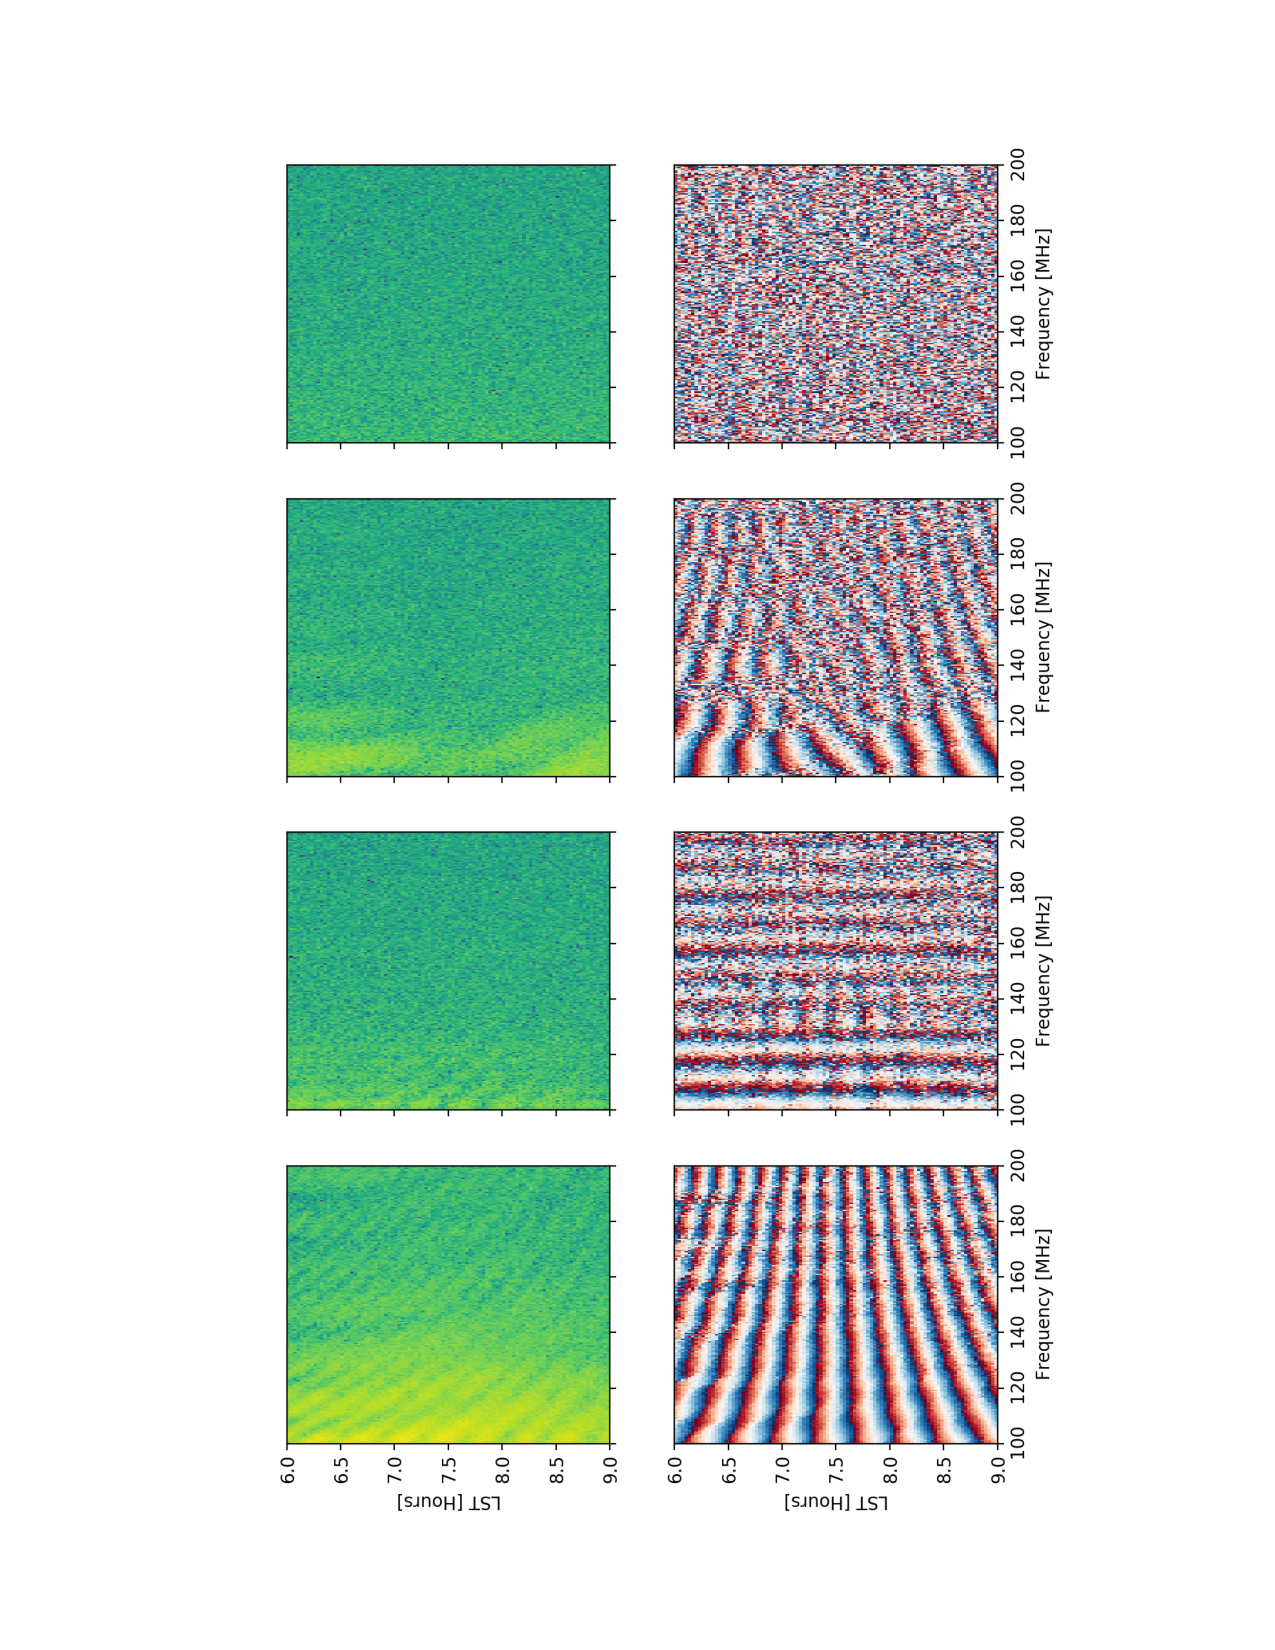
\includegraphics[width=0.6\textwidth, angle=270]{chapters/polcal/figures/sim.pdf}
\caption[Simulations of pseudo-Stokes visibilities,]{Simulations of absolute value (\textit{upper panels}) and phase (\textit{lower panels}) of pseudo-Stokes visibilities (left to right: pseudo-Stokes I, Q, U and V), as measured by a 30\,m East-West PAPER baseline. The upper group shows the noiseless simulation, and the lower shows the same simulation with the addition of a realistic PAPER noise model \citep{Moore.17}. Only a Stokes I sky was used -- all of the structure seen in $V_Q$, $V_U$ and $V_V$ can be attributed to direction-dependent leakage.}
\label{fig:simvis}
\end{figure}


\subsection{Data Processing}
\label{sec:polcal_data}

We tested these different calibration schemes on one night (JD 2456680.20 -- .65; January 22nd-23rd 2014; 6pm -- 6am South African Standard Time; Local Siderial Time 2 -- 13.5 hours) of PAPER 128-element observations. The PAPER-128 signal chain and full observation season results will be discussed in forthcoming publications, but we will provide a brief overview here. 

PAPER-128 consists of 128 dual-polarization dipole receivers, 112 of which are arranged in a highly-redundant configuration, and the rest placed as in- and outriggers to the array in order to improve \textit{uv} coverage; see Figure~\ref{fig:polcal_realarray}. Since all dipole arms are oriented North-South (`x') and East-West (`y'), \textit{xy} and \textit{yx} correlations have very low signal-to-noise compared to \textit{xx} and \textit{yy}.

All visibilities were RFI flagged using {\sc python} scripts from the {\sc aipy}\footnote{\url{https://github.com/HERA-Team/aipy}} library. These took the derivative of the frequency axis of all baselines associated with a given antenna and flagged any frequencies with a derivative 6$\sigma$ above the mean, per integration. We took the union of all baseline flags and applied them to the data. The 5\,MHz on both band-edges were always flagged. Compression proceeded as described in Appendix A of \cite{Parsons.14}, filtering to critical Nyquist sampling rates for the longest (300\,m) baseline of 493 kHz along the frequency axis (203 channels) and 42.9\,s along the time axis. 

\begin{figure}
\centering
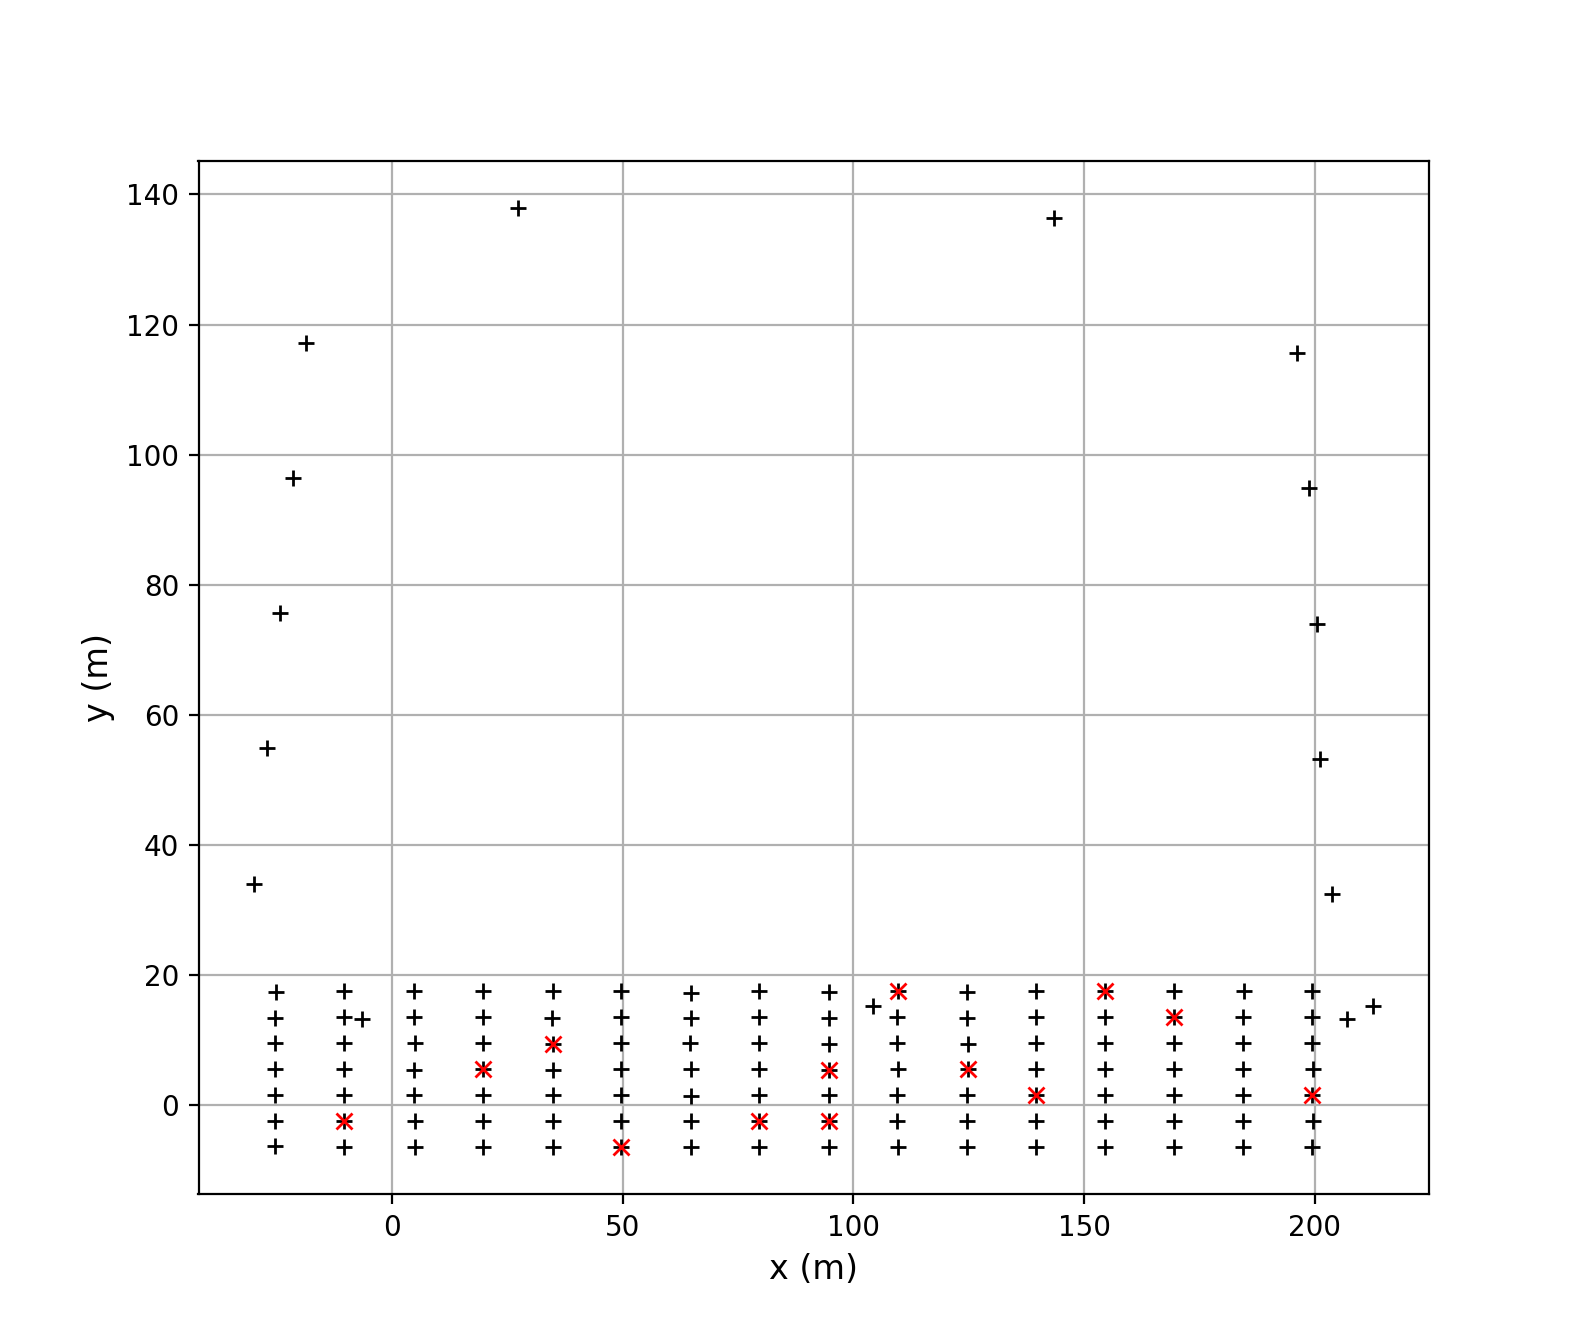
\includegraphics[scale=0.5]{chapters/polcal/figures/gridlayout.png}
\caption[Arrangement of the PAPER-128 array.]{Arrangement of the PAPER-128 array. Antennae determined to be malfunctioning are shown with red crosses and were excluded from analysis.}
\label{fig:polcal_realarray}
\end{figure}

After RFI flagging and compression, \textit{xx} and \textit{yy} visibilities were checked for erroneous behavior including 2$\sigma$ deviations from the median in number of RFI flags and mean visibility amplitude. Antennae exhibiting these behavior were excluded from further analysis (and are shown with red crosses in Figure~\ref{fig:polcal_realarray}). If an antenna qualified as `bad' in one polarization, it was excluded in all of them. Also note that we can only calibrate the 112 antennae in the redundant grid using {\sc omnical}.

For the least-squares fit to converge at the \textit{logcal} stage of calibration, visibilities cannot exhibit phase-wraps, since the system of equations solved at this stage are insensitive to additive offsets of $2\pi$ in their imaginary parts (\textit{lincal} will be able to re-insert these as required; \citealt{Liu.10}). Therefore we must flatten the phases on all visibilities prior to any implementation of {\sc omnical}. We were able to do this redundantly without reference to the sky; taking the ratio of redundant (uncalibrated) visibilities together and averaging over time, defined as:

\begin{equation}
\mathcal{V}(\nu) = \langle V_{ij, pq}(\nu,t)V^*_{kl, pq}(\nu,t) \rangle_t .
\label{eq:Vijratio}
\end{equation}

Because this is the ratio of two nominally-redundant visibilities (i.e. baselines $ij$ and $kl$ belong to the same redundant group with model visibility $V_{|i-j|,pq}$), and the measurements are not yet calibrated, we can expand Equation~\ref{eq:Vijratio} as

\begin{equation}
\mathcal{V}(\nu) = \langle g^*_{p,i}g_{q,j}g_{p,k}g^*_{q,l} |V_{|i-j|,pq}|^2 \rangle_t .
\end{equation}
Writing the complex gains as $g_{p,a}=G_{p,a} e^{-i\nu\tau_{p,a}}$ for antenna $a$, we can reduce the product of gain-amplitudes and the squared visibility into some frequency-dependent function, and an exponential product of gain phase terms

\begin{equation}
\mathcal{V}(\nu) = K(\nu)\exp\left(i\nu (\tau_i - \tau_j - \tau_k + \tau_l)\right) .
\end{equation}
A Fourier transform along the frequency axis (which we term a \textit{delay transform}; \citealt{Parsons.12a}) of $\mathcal{V}(\nu)$ gave a function that was sharply-peaked at a given delay

\begin{equation}
\tilde{\mathcal{V}}(\tau) = \tilde{K}(\tau)*\delta_D\left(\nu (\tau_i - \tau_j - \tau_k + \tau_l)\right).
\end{equation}
We can define a variable as the maximum of the above function:

\begin{equation}
\mathcal{T}_{ijkl}(\tau) = {\tt max} | \tilde{\mathcal{V}}(\tau) |,
\end{equation}
which will occur at value 

\begin{equation}
\tau = \tau_{\rm max} = \nu (\tau_i - \tau_j - \tau_k + \tau_l).
\end{equation}
With enough redundant baselines involving antennae $i,j,k$ \& $l$ this is a linearly-solvable set of equations for each value of $\tau$. Multiplying $V_{ij}$ by $e^{-2\pi i \nu (\tau_i - \tau_j)}$ by definition flattened the phase across the band. This method was very sensitive to signal-to-noise, so these initial phase estimates were created with $p=q$; that is \textit{xx} and \textit{yy} visibilities only. The estimates were then applied to all visibilities appropriately. We could then run {\sc omnical} according to each of the schemes described in Section~\ref{subsec:calSchemes}.

\subsection{Results}
\label{sec:polcal_results}

We ran {\sc omnical} using the \textit{2pol}, \textit{4pol} and \textit{4pol+minV} schemes, which granted complex gain values for each antenna feed in the redundant grid. In this work we chose to concentrate our analysis on the 30\,m East-West spacings used for PAPER power spectrum studies.

\subsubsection{Calibration}

The complex-gains dataset alone was highly multidimensional. We chose to analyze short time- and frequency- averages for these data. For example, the $\langle | g^{\rm 2pol}_{x,a} | \rangle_{t,\nu}$ notation indicates the average of the absolute value of the gain value for antenna $a$, polarization `x' in the \textit{2pol} calibration scheme. The average is over 10 minutes (the length of a single {\sc miriad} file produced by the PAPER correlator) and a 10\,MHz band running from 145 to 155 MHz (the center of the PAPER band, generally clear of RFI and used for power spectrum analyses).

Figure~\ref{fig:4pol-geo-angle} shows $\langle {\rm arg}( g^{\rm 2pol}_{a} ) \rangle_{t,\nu}$, the average phase of the gain calibration for `x' and `y' polarizations. It very clearly shows the phase-slope degeneracy present for both dipole orientations, sloping in opposite directions. 

\begin{figure}
\centering
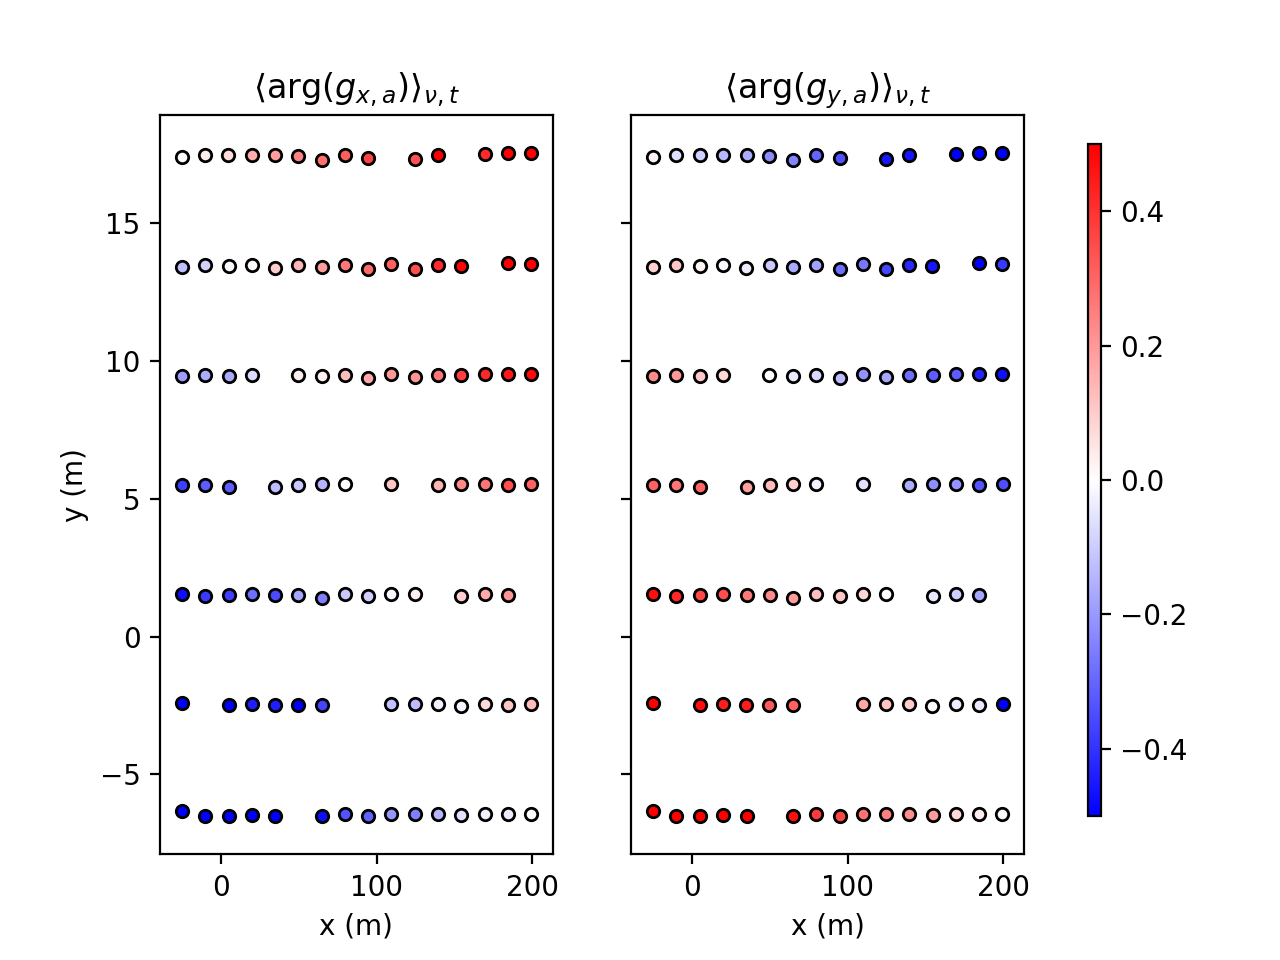
\includegraphics[scale=0.5]{chapters/polcal/figures/4pol_geo.png}
\caption[The phase of the complex gain value for the \textit{4pol} calibration scheme.]{The phase of the complex gain value for the \textit{4pol} calibration scheme is shown on the color axis (radians) for the redundant grid. The phase of the `x' gains is shown on the left, and the `y' gains on the right. The phase-slope degeneracy is clear in both panels, as is the fact that the slope is in opposite directions for the two dipole orientations.}
\label{fig:4pol-geo-angle}
\end{figure}

Figure~\ref{fig:diff-gains} shows the differences in `x' gain solutions between calibration schemes. 
The difference between \textit{4pol} and \textit{4pol+minV} was consistently smaller than the difference of either of these with the \textit{2pol} scheme. 

As noted in Section~\ref{subsubsec:degen}, {\sc omnical} tries to fix the average gain amplitude over the array to unity to avoid drifts in the amplitude degeneracy from sample to sample, so we can compare amplitude calibrations in terms of percentage deviation. The average difference in gain amplitude per antenna between \textit{2pol} and \textit{4pol} was 3.5\%, between \textit{2pol} and \textit{4pol+minV} was 2.9\%, and was 0.7\% between \textit{4pol} and \textit{4pol+minV}. The $\sim$30 degree spread in the differenced phases between the \textit{2pol} scheme and the other two is likely due to different realizations of phase degeneracies between these calibration schemes.

\begin{figure}
\centering
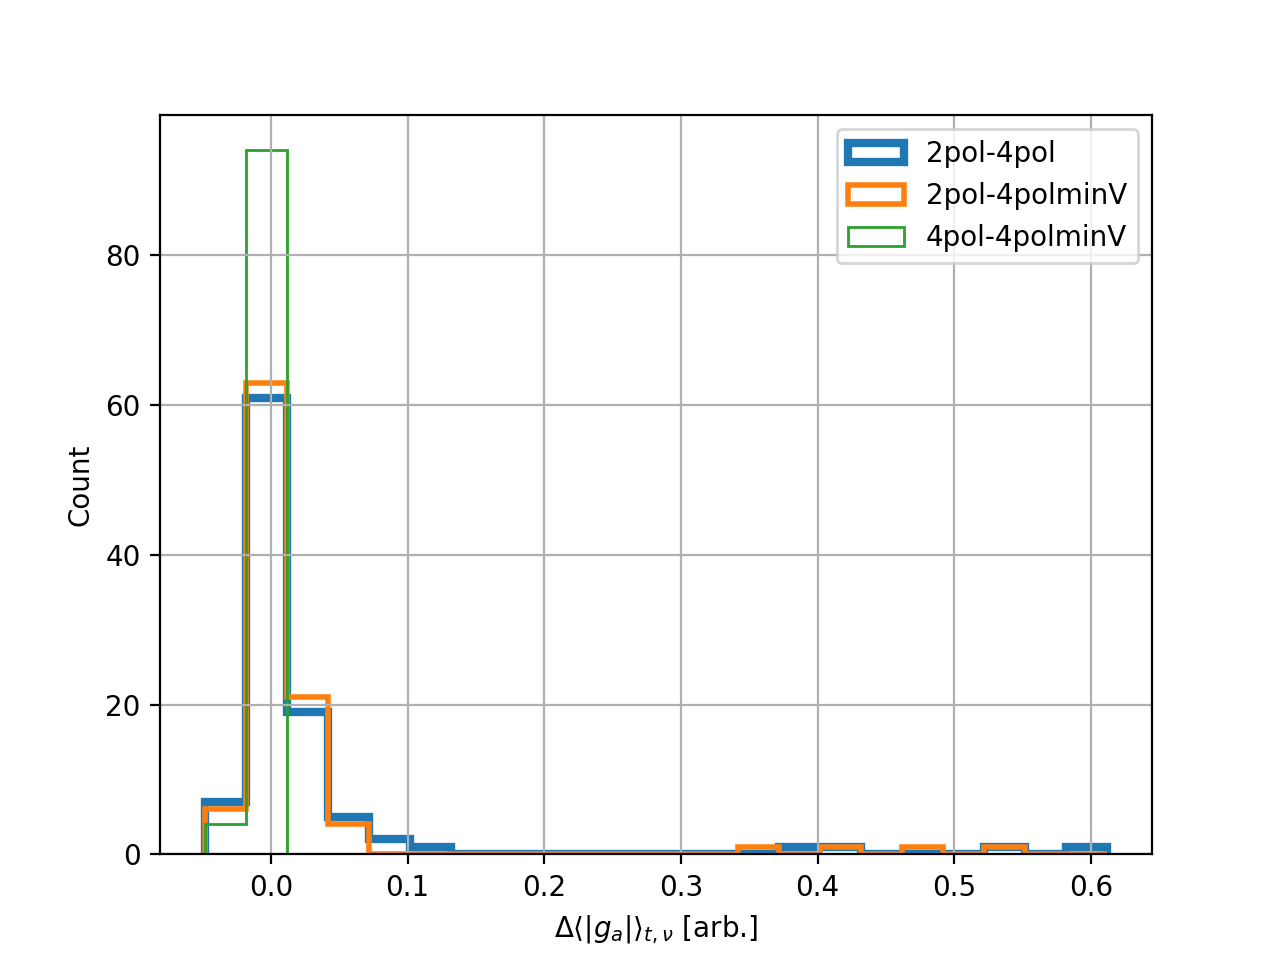
\includegraphics[scale=0.5]{chapters/polcal/figures/dGainHist.png}
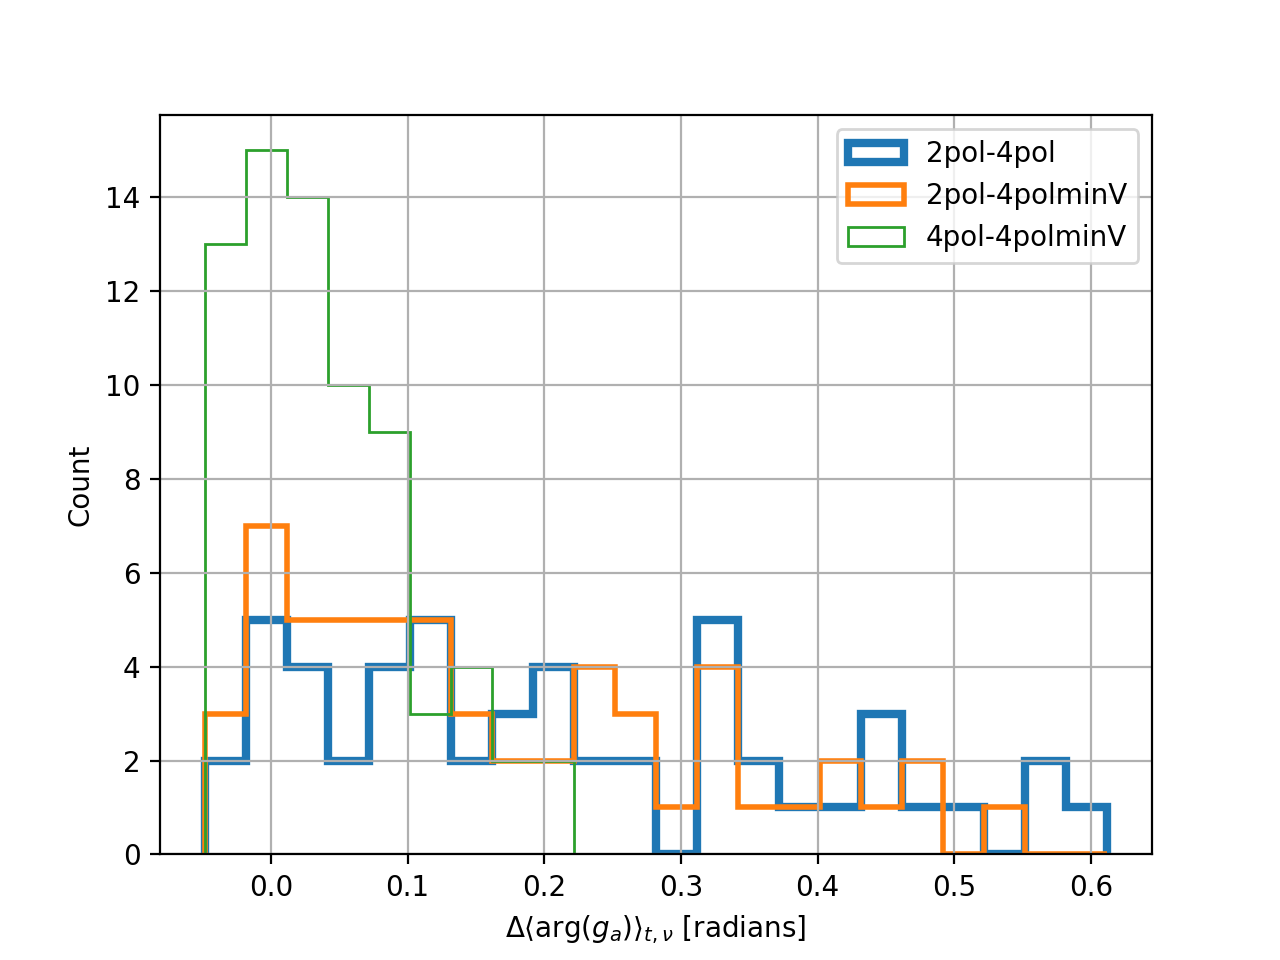
\includegraphics[scale=0.5]{chapters/polcal/figures/dAngleHist.png}
\caption[Histograms of differences in the `x' gain calibrations per antenna between calibration schemes.]{Histograms of differences in the `x' gain calibrations per antenna between calibration schemes. Above: difference in absolute value. Below: difference in phase.
For most antennae, absolute value of the gain does not change by large amounts between calibration schemes; most of the change takes place in the phase.
The difference between \textit{4pol} and \textit{4pol+minV} is consistently smaller than the difference of either of these with the \textit{2pol} scheme. This is likely a sign of different realizations of phase degeneracies between calibration schemes.}
\label{fig:diff-gains}
\end{figure}


Figure~\ref{fig:polcal_chisq} shows the sum of $w^2$ values (see Equation~\ref{eq:polcal_w2}) over all antennas in the array for each feed polarization in each of the three calibration schemes. The color scale is logarithmic. Clearly, the \textit{2pol} scheme achieves a much greater level of redundancy in each feed polarization throughout the band. Towards the end of the night, the Galaxy is in the far side-lobes of the PAPER beam and introduces higher sky temperatures, which accounts for the trend in all calibration schemes performing worse towards the end of the night. However, the reason for rapid transitions in $w^2$ at Local Sidereal Time $\sim 10.5$ in the \textit{4pol} and \textit{4pol+minV} schemes is not well understood. In general, $w^2$ is an order of magnitude higher for the \textit{4pol} and \textit{4pol+minV} schemes.

\begin{figure}
\centering
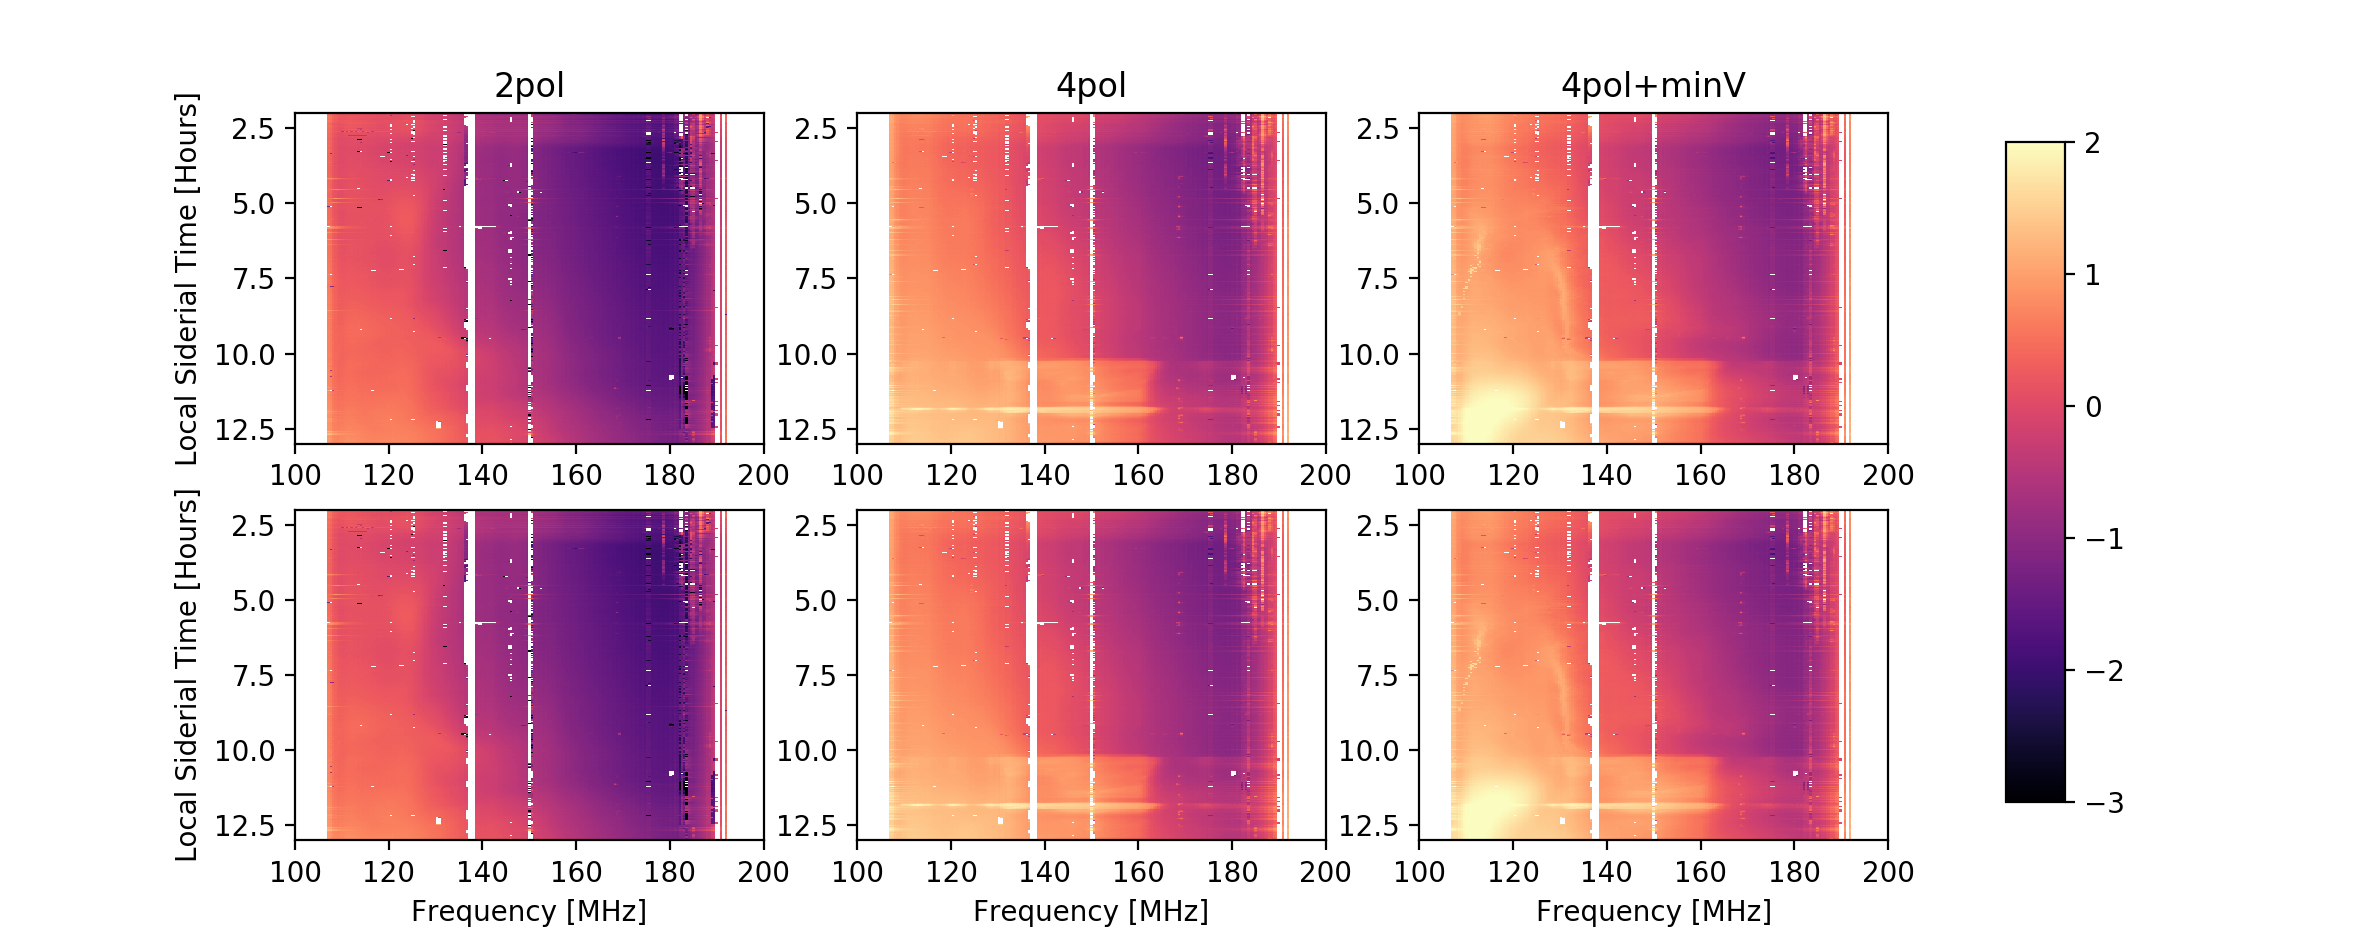
\includegraphics[width=0.75\textwidth]{chapters/polcal/figures/chisq.png}
\caption[$w^2$ values, summed across the array.]{$w^2$ values, summed across the array, for the $x$ (above) and $y$ (below) feeds in different calibration schemes. From left to right: \textit{2pol}, \textit{4pol} and \textit{4pol+minV}. The color axis is logarithmic, in arbitrary data units. The white gaps are due to RFI flagging.}
\label{fig:polcal_chisq}
\end{figure}

\subsubsection{Pseudo-Stokes Visibilities}

\subsubsection{Approximate power spectra}



\subsection{Discussion \& Conclusions}
\label{sec:polcal_disc}


\section{Imaging Calibration}
\label{sec:polcal_imagecal}

% calibrate on one field, apply to same field -- I, Q, U, V
% apply field 1 calibration to field 2 -- QUV remain noise-like
% basic-basic D-term stuff following CASA recipe




